\setcounter{chapter}{7}
\chapter{Autocorrelations and Autoregressive Models}
{\small \textit{Chapter Preview}. This chapter continues our study
of time series data. Chapter 7 introduced techniques for determining
major patterns that provide a good first step for forecasting.
Chapter 8 provides techniques for detecting subtle trends in time
and models to accommodate these trends. These techniques detect and
model relationships between the current and past values of a series
using regression concepts.}

\section{Autocorrelations}\label{S8:Autocorrs}

\empexjed{InflationBond}

\subsubsection*{Application: Inflation Bond Returns}\ecaptionjed{Inflation Bond Returns}
\index{datasets!TIPS - inflation bond returns}

To motivate the methods introduced in this chapter, we work in the
context of the inflation bond return series. Beginning in January of
2003, the US Treasury Department established an inflation bond index
that summarizes the returns on long-term bonds offered by the
Treasury Department that are inflation-indexed. For a Treasury
inflation protected security (TIPS), the principal of the bond is
indexed by the (three month lagged) value of the (non-seasonally
adjusted) consumer price index. The bond then pays a semi-annual
coupon at a rate determined at auction when the bond is issued. The
index that we examine is the unweighted average of bid yields for
all TIPS with remaining terms to maturity of 10 or more years.

Monthly values of the index from January 2003 through March 2007 are
considered, for a total of $T=51$ returns. A time series plot of the
data is presented in Figure \ref{F8:InfBondTS}. This plot suggests
that the series is stationary and so it is useful to examine the
distribution of the series through summary statistics that appear in
Table \ref{T8:InfBondSumStats}.

\begin{figure}[htp]
  \begin{center}
     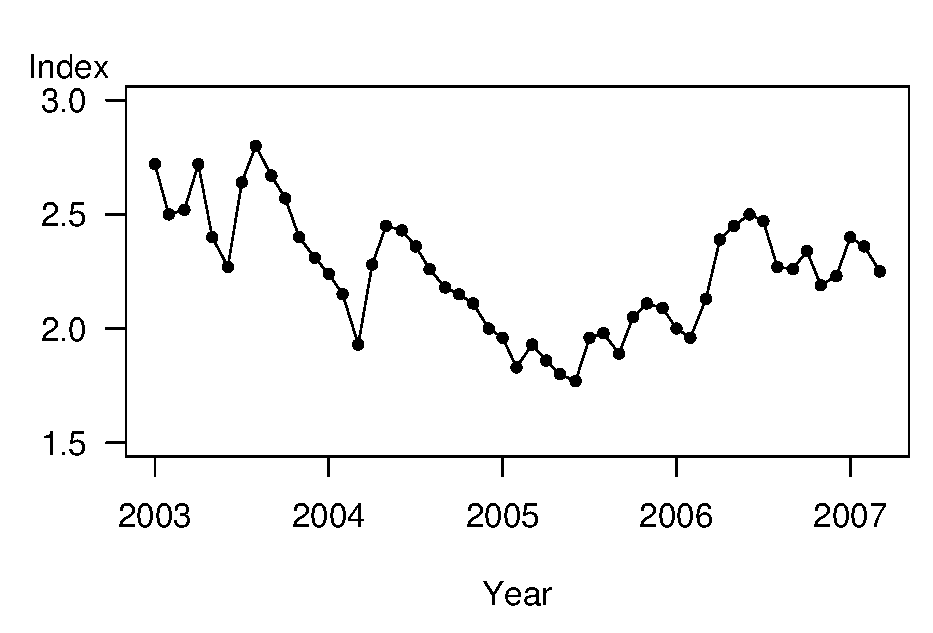
\includegraphics[width=.68\textwidth]{Chapter8AutoReg/InfBondTS.eps}
    \caption{\label{F8:InfBondTS} \small Time Series Plot of the Inflation Bond
    Index. Monthly values over January 2003 to March 2007, inclusive.}
  \end{center}
\end{figure}

\bigskip

\begin{table}[h]
\caption{\label{T8:InfBondSumStats} Summary Statistics of the
Inflation Bond Index}
\begin{center}
\begin{tabular}{lccccc}
\hline
&  &  & Standard &  &  \\
Variable & Mean & Median & Deviation & Minimum & Maximum \\ \hline
INDEX & 2.245 & 2.26 & 0.259 & 1.77 & 2.80 \\
\hline ~~~\emph{Source}: US Treasury
\end{tabular}\end{center}\end{table}

\bigskip

Our goal is detect patterns in the data and provide models to
represent these patterns. Although Figure \ref{F8:InfBondTS} shows a
stationary series with no major tendencies, a few subtle patterns
are evident. Beginning in mid 2003 and then in the beginning of
2004, we see large increases followed by a series of declines in the
index. Beginning in 2005, a pattern of increase with some cyclical
behavior seems to be occurring. Although it is not clear what
economic phenomenon these patterns represent, they are not what we
would expect to see with a white noise process. For a white noise
process, a series may increase or decrease randomly from one period
to the next, producing a non-smooth, ``jagged'' series over time.

To help understand these patterns, Figure \ref{F8:InfBondLag}
presents a scatter plot of the series ($y_t$) versus its lagged
value ($y_{t-1}$). Because this is a crucial step to understanding
this chapter, Table \ref{T8:InfBondIndex} presents a small subset of
the data so that you can see exactly what each point on the scatter
plot represents. Figure \ref{F8:InfBondLag} shows a strong
relationship between $y_t$ and $y_{t-1}$; we will model this
relationship in the next section.

\begin{figure}[htp]
  \begin{center}
    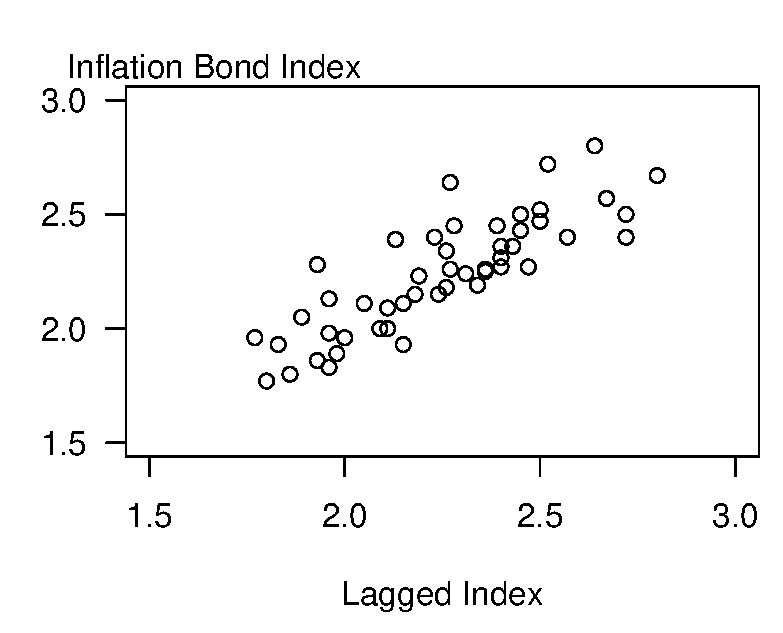
\includegraphics[width=.7\textwidth]{Chapter8AutoReg/InfBondLag.eps}
    \caption{\label{F8:InfBondLag} \small Inflation
Bond versus Lagged Value. This scatter plot reveals a linear
relationship between the index and its lagged value.}
  \end{center}
\end{figure}


\begin{table}[h]
\caption{\label{T8:InfBondIndex} Index and Lagged Index for the
First Five of $T=51$ Values}
\begin{center}
\begin{tabular}{l|rrrrr}
\hline
$t$ & 1~~ & 2~~ & 3~~ & 4~~ & 5~~ \\
Index ($y_t$) & 2.72 & 2.50 &  2.52 &  2.72 & 2.40 \\
Lagged Index ($y_{t-1}$) & * &  2.72   &  2.50   &  2.52  & 2.72
\\ \hline
\end{tabular}\end{center}\end{table}


\bigskip

\subsubsection*{Autocorrelations}\index{correlation coefficients!autocorrelations}

Scatter plots are useful because they graphically display nonlinear,
as well as linear, relationships between two variables. As we
established in Chapter 2, correlations can be used to measure the
linear relation between two variables. Recall that when dealing with
cross-sectional data, we summarized
relations between \{$y_t$\} and \{$x_t$\} using the correlation statistic%
\begin{equation*}
r = \frac{1}{(T-1)s_{x}s_y} \sum_{t=1}^{T} \left( x_t -
\overline{x}\right) \left( y_t-\overline{y} \right) .
\end{equation*}
We now mimic this statistic using the series \{$y_{t-1}$\} in place
of \{$x_t$\}. With this replacement, use $\overline{y}$\ in place of
$\overline{x}$\ and, for the denominator, use $s_y$ in place of
$s_x$. With this last substitution, we have $(T-1) s_y^2 =
\sum_{t=1}^{T}(y_t-\overline{y} )^2$. Our resulting correlation
statistic is

\begin{equation*}
r_1 = \frac{\sum_{t=2}^{T} \left( y_{t-1}-\overline{y}\right) \left(
y_t- \overline{y}\right) }{\sum_{t=1}^{T} (y_t-\overline{y})^2}.
\end{equation*}
This statistic is referred to as an \emph{autocorrelation}, that is,
a correlation of the series upon itself. This statistic summarizes
the linear relationship between \{$y_t$\} and \{$y_{t-1}$\}, that
is, observations that are one time unit apart. It will also be
useful to summarize the linear relationship between observations
that are $k$ time units apart, \{$y_t$\} and \{$y_{t-k}$\}, as
follows.\bigskip

\boxedjed

\textbf{Definition.} \ The \emph{lag k autocorrelation statistic} is
\begin{equation*}
r_k = \frac{\sum_{t=k+1}^{T}\left( y_{t-k}-\overline{y}\right) \left( y_t-%
\overline{y}\right) }{\sum_{t=1}^{T}(y_t-\overline{y})^2},
~~~~k=1,2, \ldots
\end{equation*}\index{time
series statistics!lag $k$ autocorrelation}


\end{boxedminipage}
\bigskip

Properties of autocorrelations are similar to correlations. Just as
with the usual correlation statistic $r$, the denominator,
$\sum_{t=1}^{T}(y_t - \overline{y})^2$, is always nonnegative and
hence does not change the sign of the numerator. We use this
rescaling device so that $r_k$ always lies within the interval [-1,
1]. Thus, when we interpret $r_k$, a value near -1, 0 and 1, means,
respectively, a strong negative, near null or strong positive
relationship between $y_t$ and $y_{t-k}$. If there is a positive
relationship between \ $y_t$ and $y_{t-1}$, then $r_1 > 0$ and the
process is said to be \emph{positively autocorrelated}. For example,
in Table \ref{T8:InfBondAutocorrs} are the first five
autocorrelations of the inflation bond series. These
autocorrelations indicate that there is a positive relationship
between adjacent observations.

\begin{table}[h]
\caption{\label{T8:InfBondAutocorrs} Autocorrelations for the
Inflation Bond Series}
\begin{center}
\begin{tabular}{c|ccccc}
\hline
Lag $k$ & 1 & 2 & 3 & 4 & 5 \\
Autocorrelation $r_k$ & 0.814 & 0.632 & 0.561 & 0.447 & 0.267 \\
\hline
\end{tabular}\end{center}\end{table}


\section{Autoregressive Models of Order One}
\index{time series models!autoregressive model of order one,
$AR$(1)}


\subsubsection*{Model Definition and Properties}

In Figure \ref{F8:InfBondLag} we noted the strong relationship
between the immediate past and current values of the inflation bond
index. This suggests using $y_{t-1}$ to explain $y_t$ in a
regression model. Using previous values of a series to predict
current values of a series is termed, not surprisingly, an
\emph{autoregression}. When only the immediate past is used as a
predictor, we use the following model.\bigskip

\boxedjed

\textbf{Definition.} \ The \emph{autoregressive model of order one}, denoted
by $AR(1)$, is written as%
\begin{equation}\label{E8:AR1}
y_t = \beta_0 + \beta_1 y_{t-1} + \varepsilon_t,\text{ \ \ \ \ \ \ \
\ } t=2,\ldots,T,
\end{equation}
where \{$\varepsilon_t$\} is a white noise process such that
$\mathrm{Cov}(\varepsilon_{t+k}, y_t)=0$ for $k>0$ and $\beta_0$ and
$\beta_1$ are unknown parameters.

\end{boxedminipage}
\bigskip

In the $AR$(1) model, the parameter $\beta_0$ may be any fixed
constant. However, the parameter $\beta_1$ is restricted to be
between -1 and 1. By making this restriction, it can be established
that the $AR$(1) series \{$y_t$\} is stationary. Note that if
$\beta_1 = 1$, then the model is a random walk and hence is
nonstationary. This is because, if $\beta_1 = 1$, then equation
(\ref{E8:AR1}) may be rewritten as
\begin{equation*}
y_t - y_{t-1} = \beta_0 + \varepsilon_t.
\end{equation*}
If the difference of a series forms a white noise process, then the series
itself must be a random walk.

\marginparjed{For stationarity in the $AR$(1) model, we require
$|\beta_1|<1.$}

The equation (\ref{E8:AR1}) is useful in the discussion of model
properties. We can view an $AR$(1) model as a generalization of both
a white noise process and a random walk model. If $\beta_1=0$, then
equation (\ref{E8:AR1}) reduces to a white noise process. If
$\beta_1 = 1,$ then equation (\ref{E8:AR1}) is a random walk.

A stationary process where there is a linear relationship between
$y_{t-2}$ and $y_t$ is said to be \emph{autoregressive of order 2},
and similarly for higher order processes. Discussion of higher order
processes is in Section \ref{S8:BoxJenkins}.

\subsubsection*{Model Selection}

When examining the data, how does one recognize that an
autoregressive model may be a suitable candidate model? First, an
autoregressive model is stationary and thus a control chart is a
good device to examine graphically the data to search for stability.
Second, adjacent realizations of an $AR$(1) model should be related;
this can be detected visually by a scatter plot of current versus
immediate past values of the series. Third, we can recognize an
$AR$(1) model through its autocorrelation structure, as follows.

A useful property of the $AR$(1) model is that the correlation
between points $k$ time units apart turns out to be $\beta_1^{k}$.
Stated another way,
\begin{equation}\label{E8:AR1Autocorrelations}
\rho_k = \mathrm{Corr}(y_t,y_{t-k}) =
\frac{\mathrm{Cov}(y_t,y_{t-k})}{\sqrt{\mathrm{Var}(y_t)\mathrm{Var}(y_{t-k})}}
= \frac{\mathrm{Cov}(y_t,y_{t-k})}{\sigma_y^2} = \beta_1^k.
\end{equation}
\marginparjed{For a (stationarity) $AR$(1) model, $\rho_k =\beta_1
^k .$}


\noindent The first two equalities are definitions and the third is
due to the stationarity. The reader is asked to check the fourth
equality in the exercises. Hence, the absolute values of the
autocorrelations of an $AR$(1) process become smaller as the lag
time $k$ increases. In fact, they decrease at a geometric rate. We
remark that for a white noise process, we have $\beta_1 = 0$, and
thus $\rho_k$ should be equal to zero for all lags $k$.

As an aid in model identification, we use the idea of matching the
observed autocorrelations $r_k$ to quantities that we expect from
the theory, $\rho_k$. For white noise, the sample autocorrelation
coefficient should be approximately zero for each lag $k$. Even
though $r_k$ is algebraically bounded by -1 and 1, the question
arises, how large does $r_k$ need to be, in absolute value, to be
considered significantly different from zero? The answer to this
type of question is given in terms of the statistic's standard
error. Under the hypothesis of no autocorrelation, a good
approximation to the standard error of the lag $k$ autocorrelation
statistic is
\begin{equation*}
se(r_k) = \frac{1}{\sqrt{T}}.
\end{equation*}
Our rule of thumb is that if $r_k$ exceeds $2 \times se(r_k)$ in
absolute value, it may be considered to be significantly non-zero.
This rule is based on a 5\% level of significance.

\linejed \index{datasets!TIPS - inflation bond returns}

\textbf{Example: Inflation Index Bonds - Continued.} Is a white
noise process model a good candidate to represent this series? The
autocorrelations are given in Table \ref{T8:InfBondIndex}. For a
white noise process model, we expect each autocorrelation $r_k$ to
be close to zero but note that, for example, $r_1=0.814$. Because
there are $T=51$ returns available, the approximate standard error
of each autocorrelation is
\begin{equation*}
se(r_k) = \frac{1}{\sqrt{51}} = 0.140.
\end{equation*}
Thus, $r_1$ is 0.814 / 0.140 = 5.81 standard errors above zero.
Using the normal distribution as a reference base, this difference
is significant, implying that a white noise process is not a
suitable candidate model.

Is the autoregressive model of order one a suitable choice? Well,
because $\rho_k$ = $\beta_1^{k}$, a good estimate of
$\beta_1$=$\rho_1$ is $r_1=0.814$. If this is the case, then under
the $AR$(1) model, another estimate of $\rho_k$ is $(0.814)^{k}$.
Thus, we have two estimates of $\rho_k$; (i) $r_k$, an empirical
estimate that does not depend on a parametric model and (ii)
$(r_1)^{k}$, that depends on the $AR$(1) model. To illustrate, see
Table \ref{T8:InfBondAutoEstimated}.



\begin{table}[h]
\begin{center}
\caption{\label{T8:InfBondAutoEstimated} Comparison of Empirical
Autocorrelations to Estimated under the $AR$(1) model}
\begin{tabular}{l|ccccc}
\hline
Lag $k$ & 1 & 2 & 3 & 4 & 5 \\
Estimated $\rho_k$ under the $AR$(1) model & $0.814$ & $(0.814)^2$ & $%
(0.814)^{3}$ & $(0.814)^{4}$ & $(0.814)^{5}$ \\
&  & \multicolumn{1}{r}{$=.66$} &
\multicolumn{1}{r}{$=.54$} & \multicolumn{1}{r}{$=.44$} & \multicolumn{1}{r}{%
$=.36$} \\
Autocorrelation $r_k$ & $0.814$ & $0.632$ & $0.561$ & $0.447$ & $0.267$ \\
\hline
\end{tabular}\end{center}\end{table}


\bigskip

Given that the approximate standard error is $se(r_k) = 0.14$, there
seems to be a good match between the two sets of autocorrelations.
Because of this match, in Section \ref{S8:Estimation} we will
discuss how to fit the $AR$(1) model to this set of data.

\linejed

\subsubsection*{Meandering Process}\index{time series terms and concepts!meandering
process}

Many processes display the pattern of adjacent points being related
to one another. Thinking of a process evolving as a river, Roberts
(1991) picturesquely describes such processes as \emph{meandering}.
To supplement this intuitive notion, we say that a process is
meandering if the lag one autocorrelation of the series is positive.
For example, from the plots in Figures \ref{F8:InfBondTS} and
\ref{F8:InfBondLag}, it seems clear that the Inflation Bond Index is
a good example of a meandering series. Indeed, an $AR$(1) model with
a positive slope coefficient is a meandering process.

What about the case when the slope coefficient approaches one,
resulting in a random walk? Consider the Hong Kong Exchange Rates
example given in Chapter 7. Although introduced as a quadratic trend
in time model, an exercise shows that the series can more
appropriately be modeled as a random walk. It seems clear that any
point in the process is highly related to each adjacent point in the
process. To emphasize this point, Figure \ref{F8:HKLag} shows a
strong linear relationship between the current and immediate past
value of exchange rates. Because of the strong linear relationship
in Figure \ref{F8:HKLag}, we will use the terminology ``meandering
process'' for a data set that may be modeled using a random walk.

\begin{figure}[htp]
  \begin{center}
   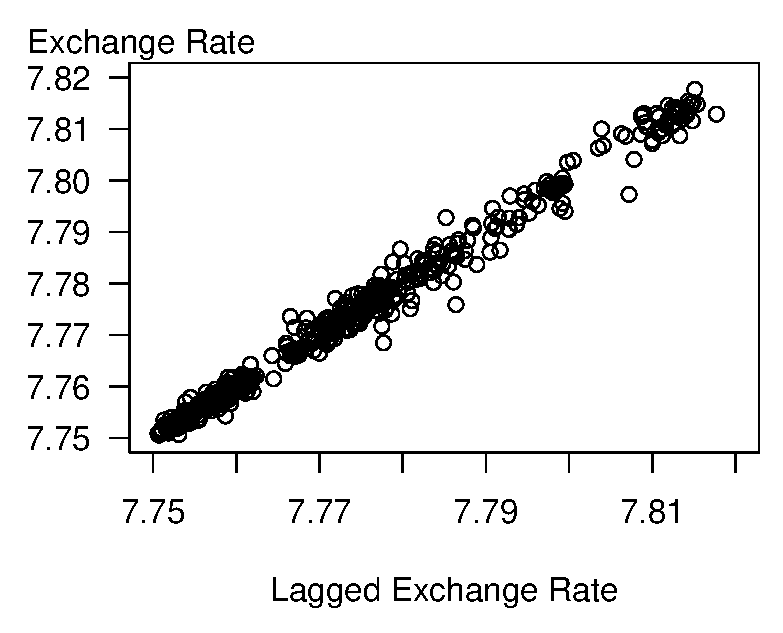
\includegraphics[width=.5\textwidth]{Chapter8AutoReg/HKLag.eps}
    \caption{\label{F8:HKLag} \small Hong Kong Daily Exchange Rates versus Lagged Values.}
  \end{center}
\end{figure}

\section{Estimation and Diagnostic Checking}\label{S8:Estimation}

Having identified a tentative model, the task now at hand is to
estimate values of $\beta_0$ and $\beta_1$. In this section, we use
the \emph{method of conditional least squares} to determine the
estimates, denoted as $b_0$ and $b_1$, respectively. This approach
is based on the least squares method that was introduced in Section
2.1. Specifically, we now use the least squares to find estimates
that best fit an observation \emph{conditional} on the previous
observation.

Formulas for the conditional least squares estimates are determined
from the usual least squares procedures, using the lagged value of
$y$ for the explanatory variable. It is easy to see that conditional
least squares estimates are closely approximated by
\begin{equation*}
b_1 \approx r_1 \text{ \ \ \ \ \ \ and \ \ \ \ \ \ }b_0 \approx
\overline{y}(1-r_1).
\end{equation*}
Differences between these approximations and the conditional least
squares estimates arise because we have no explanatory variable for
$y_1$, the first observation. These differences are typically small
in most series and diminish as the series length increases.

Residuals of an $AR$(1) model are defined as
\begin{equation*}
e_t = y_t - \left( b_0 + b_1 y_{t-1} \right).
\end{equation*}
As we have seen, patterns in the residuals may reveal ways to
improve the model specification. One can use a control chart of the
residuals to assess the stationarity and compute the autocorrelation
function of residuals to verify the lack of milder patterns through
time.

The residuals also play an important role in estimating standard
errors associated with model parameter estimates. From equation
(\ref{E8:AR1}), we see that the unobserved errors are driving the
updating of the new observations. Thus, it makes sense to focus on
the variance of the errors and, as in cross-sectional data, we
define $\sigma^2=\sigma_{\varepsilon }^2=
\mathrm{Var}~\varepsilon_t.$

In cross-sectional regression, because the predictor variables were
non-stochastic, the variance of the response ($\sigma_y^2$) equals
the variance of the errors ($\sigma^2$). This is not generally true
in time series models that use stochastic predictors. For the
$AR$(1) model, taking variances of both sides of equation
(\ref{E8:AR1}) establishes
\begin{equation*}
\sigma_y^2 (1-\beta^2) = \sigma^2 ,
\end{equation*}
so that $\sigma_y^2 > \sigma^2$.

To estimate $\sigma^2$, we define
\begin{equation}\label{E8:MSE}
s^2 = \frac{1}{T-3}\sum_{t=2}^{T} \left( e_t -
\overline{e}\right)^2.
\end{equation}
In equation (\ref{E8:MSE}) the first residual, $e_1$, is not
available because $y_{t-1}$ is not available when $t=1$ and so the
number of residuals is $T-1$. Without the first residual, the
average of the residuals is no longer automatically zero and thus is
included in the sum of squares. Further, the denominator in the
right hand side of equation (\ref{E8:MSE}) is still the number of
observations minus the number of parameters, keeping in mind the
conditions that the ``number of observations'' is $T-1$ and the
``number of parameters'' is two. As in the cross-sectional
regression context, we refer to $s^2$ as the \emph{mean square error
(MSE)}.

\linejed\index{datasets!TIPS - inflation bond returns}

\textbf{Example: Inflation Index Bonds - Continued.} The inflation
index was fit using an $AR$(1) model. The estimated equation turns
out to be
\begin{equation*}
\begin{tabular}{llllrl}
$\widehat{INDEX}_t$ & $=$ & $0.2923$ & $+$ & $0.8727$ & $INDEX_{t-1}$ \\
{\small std~errors} &  & {\small (0.0196)} &  & {\small (0.0736)} &
\end{tabular}%
\end{equation*}%
with $s = 0.14$. This is smaller than the standard deviation of the
original series (0.259 from Table \ref{T8:InfBondSumStats}),
indicating a better fit to the data than a white noise model. The
standard errors, given in parentheses, were computed using the
method of conditional least squares. For example, the $t$-ratio for
$\beta_1$ is $0.8727/0.0736=14.9$, indicating that the immediate
past response is an important predictor of the current response.

Residuals were computed as $e_t = INDEX_t -
(0.2923+0.8727INDEX_{t-1})$. The control chart of the residuals in
Figure \ref{F8:InfBondControl} reveals no apparent patterns. Several
autocorrelations of residuals are presented in Table
\ref{T8:InfBondResidAuto}. With $T=51$ observations, the approximate
standard error is $se(r_k) = 1/ \sqrt{51} = 0.14$. The second lag
autocorrelation is approximately -2.3 standard errors from zero and
the others are smaller, in absolute value. These values are lower
than those in Table \ref{T8:InfBondAutocorrs}, indicating that we
have removed some of the temporal patterns with the \textit{AR}(1)
specification. The statistically significant autocorrelation at lag
2 indicates that there is still some potential for model
improvement.\index{plots!control chart}


\begin{figure}[htp]
  \begin{center}
    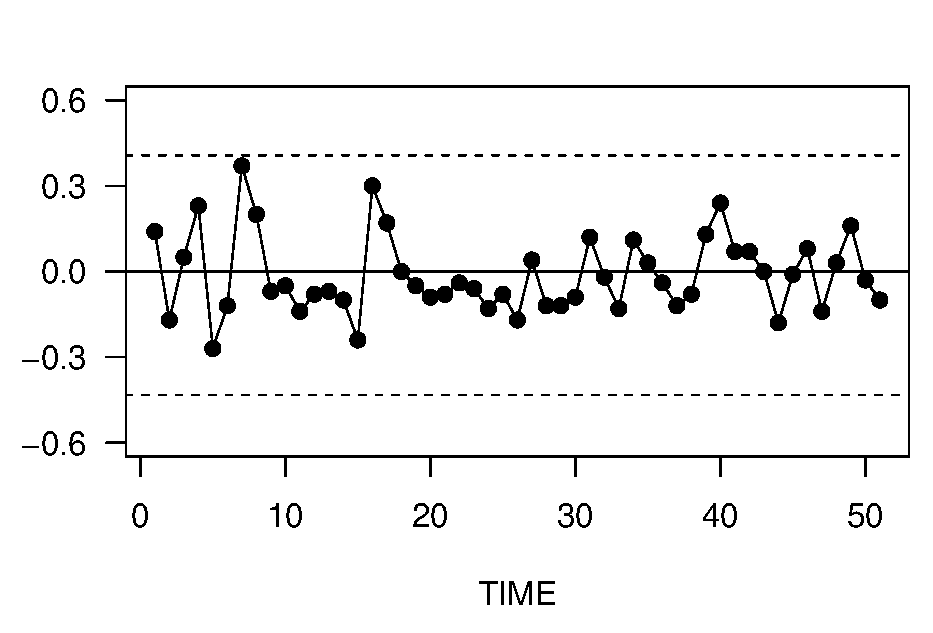
\includegraphics[width=.8\textwidth]
        {Chapter8AutoReg/InfBondControl.eps}
    \caption{\label{F8:InfBondControl} \small Control
Chart of Residuals from an ${\small AR}${\small (1) Fit of the
Inflation Index Series. The dashed lines mark the upper and lower control limits which are
the mean plus and minus three standard deviations.}}
  \end{center}
\end{figure}

\bigskip

\begin{table}[h]
\caption{\label{T8:InfBondResidAuto} Residual Autocorrelations from
the $AR$(1) model}
\begin{center}
\begin{tabular}{c|ccccc}
\hline
Lag $k$ & 1 & 2 & 3 & 4 & 5 \\
Residual Autocorrelation $r_k$ & 0.09 & -0.33 & 0.07 & 0.02 & -0.17 \\
\hline
\end{tabular}\end{center}\end{table}

\linejed

\newpage

\section{Smoothing and Prediction}\label{S8:AR1Smooth}

Having identified, fit, and checked the identification of the model, we now
proceed to basic inference. Recall that by inference we mean the process of
using the data set to make statements about the nature of the world. To make
statements about the series, analysts often examine the values fitted under
the model, called the \emph{smoothed series}. The smoothed series is the
estimated expected value of the series given the past. For the $AR$(1)
model, the smoothed series is%
\begin{equation*}
\widehat{y}_t=b_0+b_1y_{t-1}.
\end{equation*}\index{time series terms and concepts!smoothed series}

In Figure \ref{F8:InfBondSmooth}, an open circle represents the
actual Inflation Bond Index and an opaque circle represents the
corresponding smoothed series. Because the smoothed series is the
actual series with the estimated noise component removed, the
smoothed series is sometimes interpreted to represent the ``real''
value of the series.

\begin{figure}[htp]
  \begin{center}
    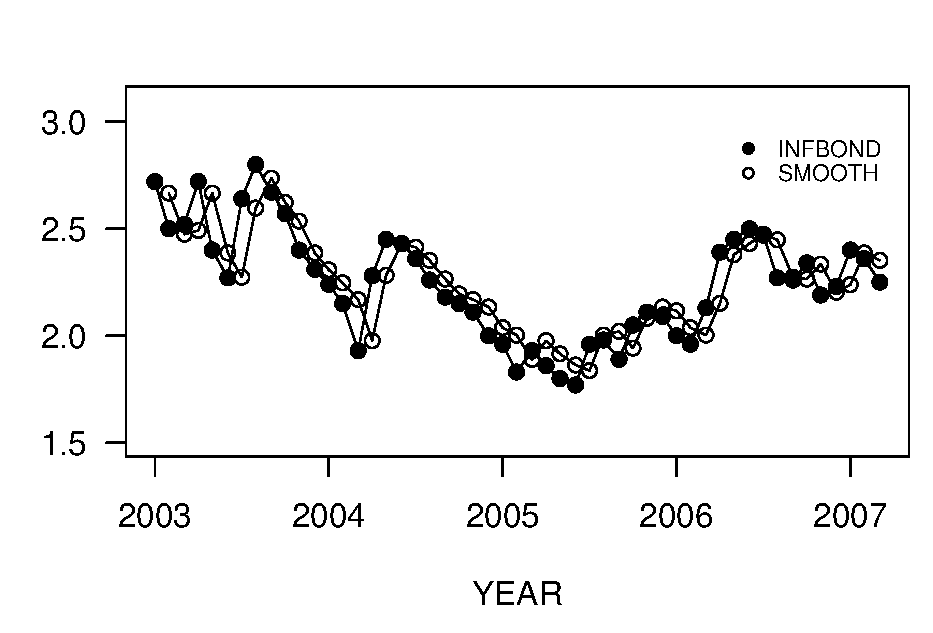
\includegraphics[width=.8\textwidth]
        {Chapter8AutoReg/InfBondSmooth.eps}
    \caption{\label{F8:InfBondSmooth} \small Inflation Bond Index with a Smoothed Series Superimposed. The
index is given by the open plotting symbols, the smoothed series is
represented by the opaque symbols.}
  \end{center}
\end{figure}

Typically, the most important application of time series modeling is
the forecasting of future values of the series. From equation
(\ref{E8:AR1}), the immediate future value of the series is $y_{T+1}
= \beta_0 + \beta_1 y_T + \varepsilon_{T+1}$. Because the series
\{$\varepsilon_t$\} is random, a natural forecast of
$\varepsilon_{T+1}$ is its mean, zero. Thus, if the estimates $b_0$
and $b_1$ are close to the true parameters $\beta_0$ and $\beta_1$,
then a desirable estimate of the series at time $T+1$ is
$\widehat{y}_{T+1} = b_0 + b_1 y_T$. Similarly, one can recursively
compute an estimate for the series $k$ time points in the future,
$y_{T+k}$. \bigskip

\boxedjed \textbf{Definition.} \ The $k$-step ahead forecast of
$y_{T+k}$ for an $AR$ (1) model is recursively determined by
\begin{equation}\label{E8:ChainRule}
\widehat{y}_{T+k} = b_0 + b_1 \widehat{y}_{T+k-1}.
\end{equation}
This is sometimes known as the \emph{chain rule of forecasting}.
\index{time series terms and concepts!chain rule of forecasting}

\end{boxedminipage}
\bigskip

To get an idea of the error in using $\widehat{y}_{T+1}$ to predict
$y_{T+1}$, assume for the moment that the error in using $b_0$ and
$b_1$ to estimate $\beta_0$ and $\beta_1$ is negligible. With this
assumption, the forecast error is
\begin{equation*}
y_{T+1}-\widehat{y}_{T+1} = \beta_0 + \beta_1 y_t +
\varepsilon_{T+1} - \left( b_0 + b_1 y_t\right) \approx
\varepsilon_{T+1}.
\end{equation*}
Thus, the variance of this forecast error is approximately
$\sigma^2$. Similarly, it can be shown that the approximate variance
of the forecast error $y_{T+k}-\widehat{y}_{T+k}$ is $\sigma^2(1 +
\beta_1^2 \ldots + \beta_1^{2(k-1)})$. From this variance
calculation and the approximate normality, we have the following
prediction interval.

\bigskip


\boxedjed

\textbf{Definition.} \ The $k$-step ahead forecast interval of
$y_{T+k}$ for an $AR$(1) model is
\begin{equation*}
\widehat{y}_{T+k} \pm (t-value)~s \sqrt{1 + b_1^2+ \ldots +
b_1^{2(k-1)}}.
\end{equation*}
Here, the $t$-value is a percentile from the $t$-curve using $df=T-3$
degrees of freedom. The percentile is 1 - (prediction level)/2.


\end{boxedminipage}
\bigskip

For example, for 95\% prediction intervals, we would have $t$-value $\approx
$ 2. Thus, one- and two-step 95\% prediction intervals are:

\begin{center}
one-step:$\qquad \widehat{y}_{T+1}\pm \ 2s$

two-step:$\qquad \widehat{y}_{T+2}\pm \ 2s(1+b_1^2)^{1/2}.$
\end{center}

Figure \ref{F8:InfBondForInt} illustrates forecasts of the inflation
bond index. The forecast intervals widen as the number of steps into
the future increases; this reflects our increasing uncertainty as we
forecast further into the future.

\begin{figure}[htp]
  \begin{center}
   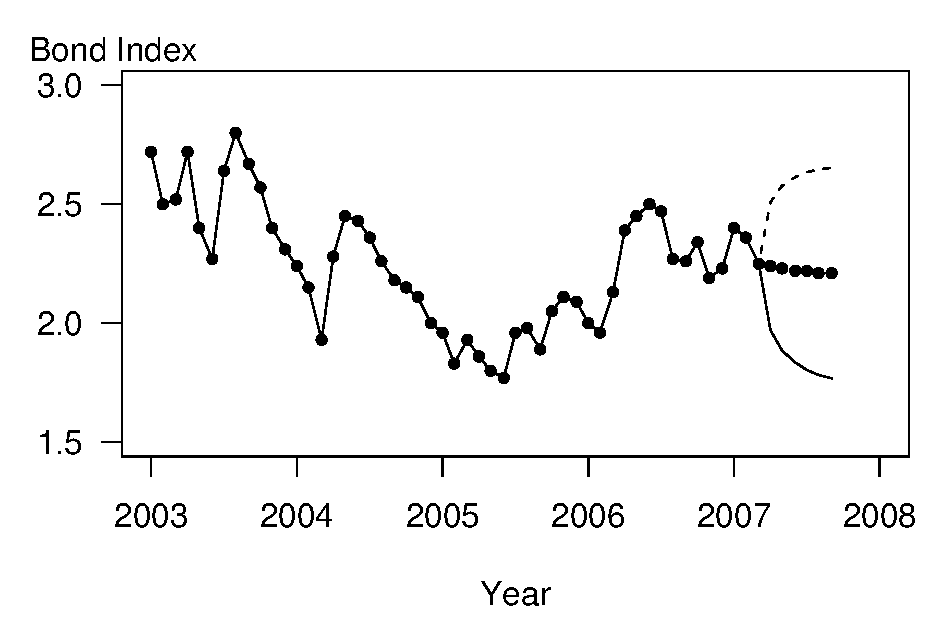
\includegraphics[width=.8\textwidth]{Chapter8AutoReg/InfBondForInt.eps}
    \caption{\label{F8:InfBondForInt} \small Forecast Intervals for the Inflation Bond Series.}
  \end{center}
\end{figure}


\section{Box-Jenkins Modeling and Forecasting}\label{S8:BoxJenkins}

Sections \ref{S8:Autocorrs} through \ref{S8:AR1Smooth} introduced
the $AR(1)$ model, including model properties, identification
methods and forecasting. We now introduce a broader class of models
known as \emph{autoregressive integrated moving average (ARIMA)
models}, due to George Box and Gwilym Jenkins, see Box, Jenkins and
Reinsel (1994).\index{time series models!autoregressive integrated
moving average ($ARIMA$) model}

\subsection{Models}

\subsubsection*{$AR(p)$ Models}\index{time series models!autoregressive model of order $p$, $AR$($p$)}


The autoregressive model of order one allows us to relate the
current behavior of an observation directly to its immediate past
value. Moreover, in some applications, there are also important
effects of observations that are more distant in the past than
simply the immediate preceding observation. To quantify this, we
have already introduced the lag $k$ autocorrelation $\rho_k$ that
captures the linear relationship between $y_t$ and $y_{t-k}$. To
incorporate this feature into a forecasting framework, we have the
\emph{autoregressive model of order p}, denoted by $AR(p).$ The
model equation is
\begin{equation} \label{E8:ARp}
y_t = \beta_0 + \beta_1 y_{t-1} + \ldots + \beta_p y_{t-p} +
\varepsilon_t, \text{ \ \ \ \ \ \ \ \ }t=p+1,\ldots ,T,
\end{equation}
where \{$\varepsilon_t$\} is a white noise process such that
$\mathrm{Cov}(\varepsilon_{t+k}, y_t)=0$ for $k>0$ and $\beta_0$,
$\beta_1,\ldots,\beta_p$ are unknown parameters.

As a convention, when data analysts specify an \textit{AR}($p$)
model, they include not only $y_{t-p}$ as a predictor variable, but
also the intervening lags, $y_{t-1}, \ldots, y_{t-p+1}$. The
exceptions to this convention are the seasonal autoregressive
models, that will be introduced in Section 9.4. Also by convention,
the $AR(p)$ is a model of a stationary, stochastic process. Thus,
certain restrictions on the parameters $\beta_1, \ldots, \beta_p$
are necessary to ensure (weak) stationarity. These restrictions are
developed in the following subsection.

\subsubsection*{Backshift Notation}
\index{time series terms and concepts!backshift operator
B}\index{symbols!B , backshift operator}

The \emph{backshift, or backwards-shift, operator} $\mathrm{B}$ is
defined by $\mathrm{B}y_t$ = $y_{t-1}$. The notation
$\mathrm{B}^{k}$ means apply the operator $k$ times, that is,
\begin{equation*}
\mathrm{B}^{k}~y_t = \mathrm{BB \cdots B~} y_t = \mathrm{B}
^{k-1}~y_{t-1} = \cdots = y_{t-k}.
\end{equation*}%
This operator is linear in the sense that $\mathrm{B} (a_1 y_t + a_2
y_{t-1}) = a_1 y_{t-1} + a_2 y_{t-2}$, where $a_1$ and $a_2$ are
constants. Thus, we can express the $AR(p)$ model as
\begin{eqnarray*}
\beta_0 + \varepsilon_t &=& y_t - \left( \beta_1 y_{t-1} + \ldots +
\beta_p y_{t-p}\right)  \\
&=& \left(1-\beta_1 \mathrm{B} - \ldots - \beta_p
\mathrm{B}^{p}\right) y_t = \Phi \left( \mathrm{B}\right) y_t.
\end{eqnarray*}
If $x$ is a scalar, then $\Phi \left( x\right) = 1 - \beta_1 x -
\ldots - \beta_p x^p$ is a $p$th order polynomial in $x$. Thus,
there exist $p$ roots of the equation $\Phi \left( x\right) =0$.
These roots, say, $g_1,..,g_p$ , may or may not be complex numbers.
It can be shown, see Box, Jenkins and Reinsel (1994), that for
stationarity, all roots lie strictly outside the unit circle. To
illustrate, for $p=1$, we have $\Phi \left( x\right) = 1 - \beta_1
x$. The root of this equation is $g_1 = \beta_1^{-1}$. Thus, we
require $|g_1|>1$, or $|\beta_1|<1$, for stationarity.

\subsubsection*{$MA(q)$ Models}\index{time series models!moving average model of order $q$, $MA$($q$)}

One interpretation of the model $y_t=\beta_0+\varepsilon_t$ is that
the disturbance $\varepsilon_t$\ perturbs the measure of the
\textquotedblleft true,\textquotedblright\ expected value of $y_t.$
Similarly, we can consider the model $y_t=\beta_0 + \varepsilon
_t-\theta_1\varepsilon_{t-1}$, where $\theta_1 \varepsilon_{t-1}$ is
the perturbation from the previous time period. Extending this line
of thought, we introduce the \emph{moving average model of order q},
denoted by
$MA(q)$. The model equation is%
\begin{equation}\label{E8:MAq}
y_t = \beta_0 + \varepsilon_t - \theta_1 \varepsilon_{t-1} - \ldots
- \theta_q \varepsilon_{t-q},
\end{equation}
where the process \{$\varepsilon_t$\} is a white noise process such
that $\mathrm{Cov}(\varepsilon_{t+k}, y_t)=0$ for $k>0$ and
$\beta_0$, $\theta_1, \ldots, \theta_q$ are unknown parameters.

With equation (\ref{E8:MAq}) it is easy to see that $\mathrm{Cov}
(y_{t+k},y_t)=0$ for $k>q$. Thus, $\rho_k =0$ for $k>q$. Unlike the
$AR(p)$ model, the $MA(q)$ process is stationary for any finite
values of the parameters $\beta_0$, $\theta_1, \ldots, \theta_q$. It
is convenient to write the $MA(q)$ using backshift notation, as
follows:
\begin{equation*}
y_t - \beta_0 = \left( 1-\theta_1\mathrm{B} - \ldots - \theta_q
\mathrm{B}^q\right) \varepsilon_t = \Theta \left( \mathrm{B}\right)
\varepsilon_t.
\end{equation*}
As with $\Phi \left( x\right) $, if $x$ is a scalar, then $\Theta
\left( x\right) = 1 - \theta_1 x - \ldots - \theta_q x^q$ is a $q$th
order polynomial in $x$. It is unfortunate that the phrase ``moving
average'' is used for the model defined by equation (\ref{E8:MAq})
and the estimate defined in Section 9.2. We will attempt to clarify
the usage as it arises.

\subsubsection*{$ARMA$ and $ARIMA$ Models}\index{time series models!autoregressive moving average ($ARMA$) model}

Combining the $AR(p)$ and the $MA(q)$ models yields the
\emph{autoregressive moving average model} of order $p$ and $q$, or
$ARMA(p,q)$,
\begin{equation}\label{E8:ARMApq}
y_t - \beta_1 y_{t-1} - \ldots - \beta_p y_{t-p} = \beta_0 +
\varepsilon _t - \theta_1 \varepsilon_{t-1} - \ldots - \theta_q
\varepsilon_{t-q},
\end{equation}
which can be represented as
\begin{equation}
\Phi \left( \mathrm{B}\right) y_t = \beta_0 + \Theta \left(
\mathrm{B} \right) \varepsilon_t.
\end{equation}

In many applications, the data requires differencing to exhibit
stationarity. We assume that the data are differenced $d$ times to
yield
\begin{equation}\label{E8:Diffd}
w_t = \left( 1-\mathrm{B}\right)^d y_t = \left( 1-\mathrm{B}\right)
^{d-1}\left( y_t-y_{t-1}\right) = \left( 1-\mathrm{B}\right)
^{d-2}\left( y_t-y_{t-1}-\left( y_{t-1}-y_{t-2}\right) \right) =
\ldots
\end{equation}
In practice, $d$ is typically zero, one or two. With this, the
\emph{autoregressive integrated moving average model} of order
$(p,d,q)$, denoted by $ARIMA(p,d,q)$, is\index{time series
models!autoregressive integrated moving average ($ARIMA$) model}
\begin{equation}
\Phi \left( \mathrm{B}\right) w_t = \beta_0+\Theta \left( \mathrm{B}
\right) \varepsilon_t.
\end{equation}
Often, $\beta_0$ is zero for $d>0$.

Several procedures are available for estimating model parameters including
maximum likelihood estimation, and conditional and unconditional least
squares estimation. In most cases, these procedures require iterative
fitting procedures. See Abraham and Ledolter (1983) for further information.

\linejed

\index{examples!Lee-Carter mortality rate forecasts}

\textbf{Example: Forecasting Mortality Rates}\ecaptionjed{Lee-Carter
Mortality Rate Forecasts}. To quantify values in life insurance and
annuities, actuaries need forecasts of age-specific mortality rates.
Since its publication, the method proposed by Lee and Carter (1992)
has proved to be a popular method to forecast mortality. For
example, Li and Chan (2007) used these methods to produce forecasts
of 1921-2000 Canadian population rates and 1900-2000 U.S. rates.
They showed how to modify the basic methodology to incorporate
atypical events including wars and pandemic events such as influenza
and pneumonia.

The Lee-Carter method is usually based on central death rates at age
$x$ at time $t$, denoted by $m_{x,t}$. The model equation is
\begin{equation}\label{E8:LeeCarter}
m_{x,t} = \alpha_x + \beta_x \kappa_t + \varepsilon_{x,t} .
\end{equation}
Here, the intercept ($\alpha_x$) and slope ($\beta_x$) depend only
on age $x$, not on time $t$. The parameter $\kappa_t$ captures the
important time effects (except for those in the disturbance term
$\varepsilon_{x,t}$).

At first glance, the Lee-Carter model appears to be a linear
regression with one explanatory variable. However, the term
$\kappa_t$ is not observed and so different techniques are required
for model estimation. Different algorithms are available, including
the singular value decomposition proposed by Lee and Carter, the
principal components approach and a Poisson regression model; see Li
and Chan (2007) for references.\index{principal components}

The time-varying term $\kappa_t$ is typically represented using an
$ARIMA$ model. Li and Chan found that a random walk (with
adjustments for unusual events) was a suitable model for Canadian
and U.S. rates (with different coefficients), reinforcing the
findings of Lee and Carter.



\linejed \bigskip



\subsection{Forecasting}

\subsubsection*{Optimal Point Forecasts}

Similar to forecasts that were introduced in Section
\ref{S8:AR1Smooth}, it is common to provide forecasts that are
estimates of conditional expectations of the predictive
distribution. Specifically, assume we have available a realization
of \{$y_1, y_2, \ldots, y_T$\} and would like to forecast $y_{T+l}$,
the value of the series ``$l$'' lead time units in the future. If
the parameters of the process were known, then we would use
$\mathrm{E}(y_{T+l}|y_T,y_{T-1},y_{T-2},\ldots)$, that is, the
conditional expectation of $y_{T+l}$ given the value of the series
up to and including time $T$. We use the notation $\mathrm{E}_T$ for
this conditional expectation.

To illustrate, taking $t=T+l$ and applying $\mathrm{E}_T$\ to both
sides of equation (\ref{E8:ARMApq}) yields
\begin{equation}\label{E8:ChainRuleForecasting}
y_T(l) - \beta_1 y_T(l-1) - \ldots - \beta_p y_T(l-p) = \beta_0 +
\mathrm{E}_T\left( \varepsilon_{T+l} - \theta_1 \varepsilon_{T+l-1}
- \ldots - \theta _q \varepsilon_{T+l-q}\right) ,
\end{equation}
using the notation $y_T(k) = \mathrm{E}_T\left( y_{T+k}\right) $.
For $k \leq 0$, $\mathrm{E}_T\left( y_{T+k}\right) =y_{T+k}$, as the
value of $y_{T+k}$\ is known at time $T$. Further,
$\mathrm{E}_T\left( \varepsilon_{T+k}\right) =0$ for $k>0$ as
disturbance terms in the future are assumed to be uncorrelated with
current and past values of the series. Thus, equation
(\ref{E8:ChainRuleForecasting}) provides the basis of the
\emph{chain rule of forecasting}, where we recursively provide
forecasts at lead time $l$ based on prior forecasts and realizations
of the series. To implement equation
(\ref{E8:ChainRuleForecasting}), we substitute estimates for
parameters and residuals for disturbance terms.\index{time series
terms and concepts!chain rule of forecasting}

\textbf{Special Case - MA(1) Model}. We have already seen the
forecasting chain rule for the $AR(1)$ model in Section
\ref{S8:AR1Smooth}. For the $MA(1)$ model, note that for $l\geq 2$,
we have $y_T(l)=\mathrm{E}_T\left( y_{T+l}\right)
=\mathrm{E}_T\left(
\beta_0+\varepsilon_{T+l}-\theta_1\varepsilon_{T+l-1}\right)
=\beta_0$, because $\varepsilon_{T+l}$\ and $\varepsilon _{T+l-1}$\
are in the future at time $T$. For $l=1$, we have $y_T(1)=
\mathrm{E}_T\left( \beta_0+\varepsilon_{T+1}-\theta
_1\varepsilon_T\right) =\beta_0-\theta_1\mathrm{E}_T\left(
\varepsilon_T\right) $. Typically, one would estimate the term
$\mathrm{E}_T\left( \varepsilon_T\right) $\ using the residual at
time $T$.


\subsubsection*{$\protect\psi $-Coefficient Representation}

Any $ARIMA(p,d,q)$ model can be expressed as%
\begin{equation*}
y_t=\beta_0^{\ast }+\varepsilon_t+\psi_1 \varepsilon_{t-1}+\psi
_2\varepsilon_{t-2}+\ldots=\beta_0^{\ast }+\sum_{k=0}^{\infty }\psi
_{k}\varepsilon_{t-k},
\end{equation*}%
called the $\psi $\emph{-coefficient representation}. That is, the
current value of a process can be expressed as a constant plus a
linear combination of the current and previous disturbances. Values
of \{$\psi_{k}$\} depend on the linear parameters of the $ARIMA$
process and can be determined via straightforward recursive
substitution. To illustrate, for the $AR(1)$ model, we have
\begin{eqnarray*}
y_t &=&\beta_0+\varepsilon_t+\beta_1y_{t-1}=\beta_0+\varepsilon
_t+\beta_1\left( \beta_0+\varepsilon
_{t-1}+\beta_1y_{t-2}\right) =\ldots \\
&=&\frac{\beta_0}{1-\beta_1}+\varepsilon_t+\beta_1\varepsilon
_{t-1}+\beta_1^2\varepsilon_{t-2}+\ldots=\frac{\beta_0}{1-\beta_1}%
+\sum_{k=0}^{\infty }\beta_1^{k}\varepsilon_{t-k}.
\end{eqnarray*}%
That is, $\psi_{k}=\beta_1^{k}$.\index{time series terms and
concepts!$\psi $-coefficient representation}

\subsubsection*{Forecast Interval}

Using the $\psi $-coefficient representation, we can express the
conditional expectation of $y_{T+l}$ as
\begin{equation*}
\mathrm{E}_T\left( y_{T+l}\right) =\beta_0^{\ast
}+\sum_{k=0}^{\infty }\psi_{k}\mathrm{E}_T\left( \varepsilon
_{T+l-k}\right) =\beta_0^{\ast }+\sum_{k=l}^{\infty }\psi
_{k}\mathrm{E}_T\left( \varepsilon_{T+l-k}\right) .
\end{equation*}
This is because, at time $T$, the errors $\varepsilon_T,\varepsilon
_{T-1},\ldots$, have been determined by the realization of the
process. However, the errors
$\varepsilon_{T+1},\ldots,\varepsilon_{T+l}$ have not been realized
and hence have conditional expectation zero. Thus, the $l$-step
forecast error is
\begin{equation*}
y_{T+l}-\mathrm{E}_T\left( y_{T+l}\right) =\beta_0^{\ast
}+\sum_{k=0}^{\infty }\psi_{k}\varepsilon_{T+l-k}-\left(
\beta_0^{\ast }+\sum_{k=l}^{\infty }\psi_{k}\mathrm{E}_T\left(
\varepsilon _{T+l-k}\right) \right)
=\sum_{k=0}^{l-1}\psi_{k}\varepsilon _{T+l-k}.
\end{equation*}

We focus on the variability of the forecasts errors. That is,
straightforward calculations yield $\mathrm{Var}\left(
y_{T+l}-\mathrm{E}_T \left( y_{T+l}\right) \right)
=\sigma^2\sum_{k=1}^{l-1}\psi_{k}^2$. Thus, assuming normality of
the errors, a $100(1-\alpha) \%$ forecast interval for $y_{T+l}$ is
\begin{equation*}
\widehat{y}_{T+l} \pm (t-value) s \sqrt{\sum_{k=0}^{l-1}
\widehat{\psi}_k^2} .
\end{equation*}
where $t$-value is the $(1-\alpha /2)^{th}$ percentile from a
$t$-distribution with $df=T-(number~of~linear~parameters)$. If $y_t$
is an $ARIMA(p,d,q)$ process, then $\psi_{k}$ is a function of
$\beta_1,\ldots,\beta_p,\theta_1,\ldots,\theta_q$ and the number of
linear parameters is $1+p+q$.

\section{Application: Hong Kong Exchange Rates}\index{datasets!Hong Kong exchange rates}\empexjed{HKExchange}

Section 7.2 introduced the Hong Kong Exchange Rate series, based on
$T=502$ daily observations for the period April 1, 2005 through Mary
31, 2007. A quadratic trend was fit to the model that produced an
$R^2=86.2\%$ with a residual standard deviation of $s=0.0068$. We
now show how to improve on this fit using $ARIMA$ modeling.

To begin, Figure \ref{F8:HKResids} shows a time series plot of
residuals from the quadratic trend time model. This plot displays a
meandering pattern, suggesting that there is information in the
residuals that can be exploited.

\begin{figure}[htp]
  \begin{center}
   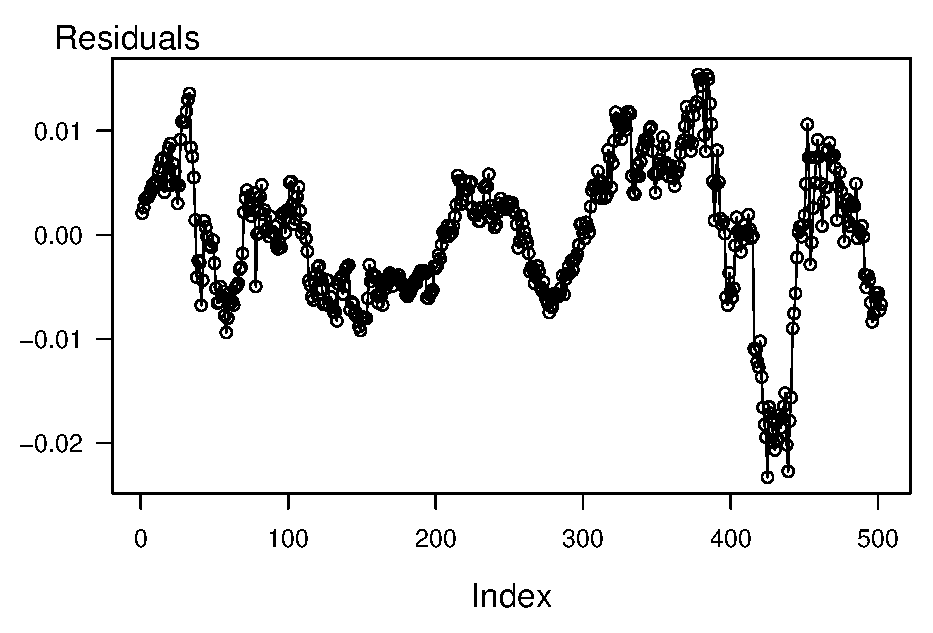
\includegraphics[width=.8\textwidth]{Chapter8AutoReg/HKResids.eps}
   \caption{\label{F8:HKResids} \small Residuals from a Quadratic Trend in Time
Model of the Hong Kong Exchange Rates.}
  \end{center}
\end{figure}



Further evidence of these patterns is in the table of
autocorrelations in Table \ref{T8:HKRatesAuto}. Here, we see large
residual autocorrelations that do not decrease quickly as the lag
$k$ increases. A similar pattern is also evident for the original
series, EXHKUS. This confirms the nonstationarity that we observed
in Section 7.2.

As an alternative transform, we differenced the series, producing
DIFFHKUS. This differenced series has a standard deviation of
$s_{DIFF}=0.0020$, suggesting that it is more stable than the
original series or the residuals from the quadratic trend in time
model. Table \ref{T8:HKRatesAuto} presents the autocorrelations from
the differenced series, indicating mild patterns. However, these
autocorrelations are still significantly different from zero. For
$T=501$ differences, we may use as an approximate standard error for
autocorrelations $1/\sqrt{501}\approx 0.0447.$ With this, we see
that the lag 2 autocorrelation is $0.151/0.0447\approx 3.38$
standard errors below zero, which is statistically significant. This
suggests introducing another model to take advantage of the
information in the time series patterns.

\bigskip

\begin{table}[h]
\scalefont{0.8}
 \caption{\label{T8:HKRatesAuto} Autocorrelations of
Hong Kong Exchange Rates}
\begin{center}
\begin{tabular}{l|cccccccccc}
\hline
Lag & 1 & 2 & 3 & 4 & 5 & 6 & 7 & 8 & 9 & 10 \\
Residuals from the & 0.958 & 0.910 & 0.876 & 0.847 & 0.819 & 0.783 & 0.748 &
0.711 & 0.677 & 0.636 \\
\ \ Quadratic Model &  &  &  &  &  &  &  &  &  &  \\
EXHKUS  & 0.988 & 0.975 & 0.963 & 0.952 & 0.942 & 0.930 & 0.919 &
0.907 & 0.895
& 0.882 \\
\ \ (Original Series) &  &  &  &  &  &  &  &  &  &  \\
DIFFHKUS & 0.078 & -0.151 & -0.038 & -0.001 & 0.095 & -0.005 & 0.051
& -0.012 & 0.084 & -0.001 \\ \hline
\end{tabular}\end{center}

\scalefont{1.25}\end{table}

\subsubsection*{Model Selection and Partial
Autocorrelations}\index{correlation coefficients!partial
autocorrelation}

\marginparjed{For stationary autoregressive models, $|\rho_k|$
becomes small as the lag $k$ increases.}

For all stationary autoregressive models, it can be shown that the
absolute values of the autocorrelations become small as the lag $k$
increases. In the case that the autocorrelations decrease
approximately like a geometric series, an \textit{AR}(1) model may
be identified. Unfortunately, for other types of autoregressive
series, the rules of thumb for identifying the series from the
autocorrelations become more cloudy. One device that is useful for
identifying the order of an autoregressive series is the
\emph{partial autocorrelation function}.

Just like autocorrelations, we now define a \emph{partial
autocorrelation} at a specific lag $k$. Consider the model equation
\begin{equation*}
y_t=\beta_{0,k}+\beta_{1,k} y_{t-1}+\ldots+\beta_{k,k} y_{t-k} +
\varepsilon_t.
\end{equation*}
Here, \{$\varepsilon_t$\} is a stationary error that may or may not
be a white noise process. The second subscript on the $\beta$'s,
``$,k$'', is there to remind us that the value of each $\beta $ may
change when the order of the model, $k$, changes. With this model
specification, we can interpret $\beta_{k,k}$ as the correlation
between $y_t$ and $y_{t-k}$ after the effects of the intervening
variables, $y_{t-1},\ldots,y_{t-k+1}$, have been removed. This is
the same idea as the partial correlation coefficient, introduced in
Section 4.4. Estimates of partial correlation coefficients,
$b_{k,k}$, can then be calculated using conditional least squares or
other techniques. As with other correlations, we may use
$1/\sqrt{T}$ as an approximate standard error for detecting
significant differences from zero.

\marginparjed{A lag k partial autocorrelation is the correlation
between $y_t$ and $y_{t-k}$, controlling for the effects of the
intervening variables, $y_{t-1},\ldots,y_{t-k+1}$.}

Partial autocorrelations are used in model identification in the following
way. First calculate the first several estimates, $b_{1,1},b_{2,2},b_{3,3}$,
and so on. Then, choose the order of the autoregressive model to be the
largest $k$ so that the estimate $b_{k,k}$ is significantly different from
zero.

To see how this applies in the Hong Kong Exchange Rate example,
recall that the approximate standard error for correlations is
$1/\sqrt{501}\approx 0.0447$. Table \ref{T8:PartialAuto} provides
the first ten partial autocorrelations for the rates and for their
differences. Using twice the standard error as our cut-off rule, we
see that the second partial autocorrelation of the differences
exceeds $2\times 0.0447=0.0894$ in absolute value. This would
suggest using an $AR(2)$ as a tentative first model choice.
Alternatively, the reader may wish to argue that because the fifth
and ninth partial autocorrelations are also statistically
significant, suggesting a more complex $AR(5)$ or $AR(9)$ would be
more appropriate. The philosophy is to ``use the simplest model
possible, but no simpler.'' We prefer to employ simpler models and
thus fit these first and then test to see whether or not they
capture the important aspects of the data.

\marginparjed{Another way of identifying a series as nonstationary
is to examine the partial autocorrelation function and look for a
large lag one partial autocorrelation.}

Finally, you may be interested to see what happens to partial
autocorrelations calculated on a non-stationary series. Table
\ref{T8:PartialAuto} provides partial autocorrelations for the
original series (EXHKUS). Note how large the first partial
autocorrelation is. That is, yet another way of identifying a series
as nonstationary is to examine the partial autocorrelation function
and look for a large lag one partial autocorrelation.


\begin{table}[h]
\scalefont{0.9} \caption{\label{T8:PartialAuto} Partial
Autocorrelations of EXHKUS and DIFFHKUS}
\begin{tabular}{c|cccccccccc}
\hline
Lag & 1 & 2 & 3 & 4 & 5 & 6 & 7 & 8 & 9 & 10 \\
EXHKUS & 0.988 & -0.034 & 0.051 & 0.019 & -0.001 & -0.023 & 0.010 &
-0.047 &
-0.013 & -0.049 \\
DIFFHKUS & 0.078 & -0.158 & -0.013 & -0.021 & 0.092 & -0.026 & 0.085
& -0.027 & 0.117 & -0.036 \\ \hline
\end{tabular}\scalefont{1.1111}
\end{table}


\subsubsection*{Residual Checking}

Having identified and fit a model, residual checking is still an important
part of determining a model's validity. For the $ARMA(p,q)$ model, we
compute fitted values as

\begin{equation}\label{E8:ARMAFittedValues}
\widehat{y}_t = b_0 + b_1 y_{t-1} + \ldots + b_p y_{t-p} -
\widehat{\theta}_1 e_{t-1}- \ldots - \widehat{\theta }_q e_{t-q}.
\end{equation}
Here, $\widehat{\theta}_1, \ldots, \widehat{\theta}_q$ are estimates
of $\theta_1,\ldots, \theta_q$. The residuals may be computed in the
usual fashion, that is, as $e_t=y_t-\widehat{y}_t$. Without further
approximations, note that the initial residuals are missing because
fitted values before time $t=\max (p,q)$ can not be calculated using
equation (\ref{E8:ARMAFittedValues}). To check for patterns, use the
devices described in Section \ref{S8:Estimation}, such as the
control chart to check for stationarity and the autocorrelation
function to check for lagged variable relationships.

\subsubsection*{Residual Autocorrelation}

Residuals from the fitted model should resemble white noise and
hence, display few discernible patterns. In particular, we expect
$r_k(e)$, the lag $k$ autocorrelation of residuals, to be
approximately zero. To assess this, we have that $se\left( r_k(e)
\right) \approx 1/\sqrt{T}$. More precisely, MacLeod (1977, 1978)
has given approximations for a broad class of $ARMA$ models. It
turns out that the $1/\sqrt{T}$ can be improved for small values of
$k$. (These improved values can be seen in the output of most
statistical packages.) The improvement depends on the model that is
being fit. To illustrate, suppose that an $AR(1)$ model with
autoregressive parameter $\beta_1$ is fit to the data. Then, the
approximate standard error of the lag one residual autocorrelation
is $|\beta_1|/\sqrt{T}$ . This standard error can be much smaller
than $1/\sqrt{T}$, depending on the value of $\beta_1$.

\subsubsection*{Testing Several Lags}

To test whether there is significant residual autocorrelation at a
specific lag $k$, we use $r_k(e) /se\left( r_k(e) \right)$. Further,
to check whether residuals resemble a white noise process, we might
test whether $r_k(e)$ is close to zero for several values of $k$. To
test whether the first $K$ residual autocorrelation are zero, use
the Box and Pierce (1970) chi-square statistic\index{time series
statistics!Box-Pierce chi-square}\index{distributions!chi-square}
\begin{equation*}
Q_{BP} = T \sum_{k=1}^{K} r_k \left( e \right)^2.
\end{equation*}
Here, $K$ is an integer that is user-specified. If there is no real
autocorrelation, then we expect $Q_{BP}$ to be small; more
precisely, Box and Pierce showed that $Q_{BP}$ follows an
approximate $\chi^2$ distribution with
$df=K-(number~of~linear~parameters)$. For an $ARMA(p,q)$ model, the
number of linear parameters is $1+p+q.$ Another widely used
statistic is
\begin{equation*}
Q_{LB}=T(T+2)\sum_{k=1}^{K}\frac{r_k \left( e\right)^2}{T-k}.
\end{equation*}
\marginparjed{Appendix A3.2 provides additional details about the
chi-square distribution, including a graph and percentiles.}

\noindent due to Ljung and Box (1978). This statistic performs
better in small samples than the $BP$ statistic. Under the
hypothesis of no residual autocorrelation, $Q_{LB}$ follows the same
$\chi^2$ distribution as $Q_{BP}$. Thus, for each statistic, we
reject $H_{0}$: No Residual Autocorrelation if the statistic exceeds
$chi$-value, a $1-\alpha$ percentile from a $\chi^2$ distribution. A
convenient rule of thumb is to use $chi$-value = 1.5
$df.$\index{time series statistics!Box-Ljung chi-square}

\linejed\index{datasets!Hong Kong exchange rates}

\textbf{Example: Hong Kong Exchange Rate - Continued.} Two models
were fit, the $ARIMA(2,1,0)$ and the $ARIMA(0,1,2)$; these are the
$AR(2)$ and $MA(2)$ models after taking differences. Using \{$y_t$\}
for the differences, the estimated $AR(2)$ model is:
\begin{equation*}
\begin{tabular}{clllrllll}
$\widehat{y}_t$ & $=$ & $0.0000317$ & $+$ & $0.0900$ & $y_{t-1}$ & $-$ & $%
0.158$ & $y_{t-2}$ \\
\multicolumn{1}{l}{\small $t$-statistic} &  &
\multicolumn{1}{c}{\small [0.37]} &  & \multicolumn{1}{c}{\small
[2.03]} &
 & & \multicolumn{1}{c}{\small
[-3.57]} &
\end{tabular}
\end{equation*}
with a residual standard error of $s=0.00193.$ The estimated $MA(2)$
is:
\begin{equation*}
\begin{tabular}{clllrllll}
$\widehat{y}_t$ & $=$ & $0.0000297$ & $-$ & $0.0920$ & $e_{t-1}$ & $+$ & $%
0.162$ & $e_{t-2}$ \\
\multicolumn{1}{l}{\small $t$-statistic} &  &
\multicolumn{1}{c}{\small [0.37]} & & \multicolumn{1}{c}{\small
[-2.08]} & &  & \multicolumn{1}{c}{\small [3.66]} &
\end{tabular}
\end{equation*}
with the same residual standard error of $s=0.00193.$ These
statistics indicate that the models are roughly comparable. The
Ljung-Box statistic in Table \ref{T8:HKRatesLB} also indicates a
great deal of similarity for the models.

\bigskip

\begin{table}[h]
\caption{\label{T8:HKRatesLB} Ljung-Box Statistics $Q_{LB}$ for Hong
Kong Exchange Rate Models}
\begin{tabular}{lccccc}
\hline
& \multicolumn{5}{c}{Lag $K$} \\
Model  & 2 & 4 & 6 & 8 & 10 \\  \hline
$AR(2)$ & 0.0050 & 0.5705 & 6.3572 & 10.4746 & 16.3565 \\
$MA(2)$ & 0.0146 & 0.2900 & 6.6661 & 11.3655 & 17.7326 \\ \hline
\end{tabular}
\end{table}

The fitted $MA$(2) and $AR$(2) models are roughly similar. We
present the $AR$(2) model for forecasting only because
autoregressive models are typically easier to interpret. Figure
\ref{F8:HKForecast} summarizes the predictions, calculated for ten
days. Note the widening forecast intervals, typical of forecasts for
nonstationary series.
\begin{figure}[htp]
  \begin{center}
    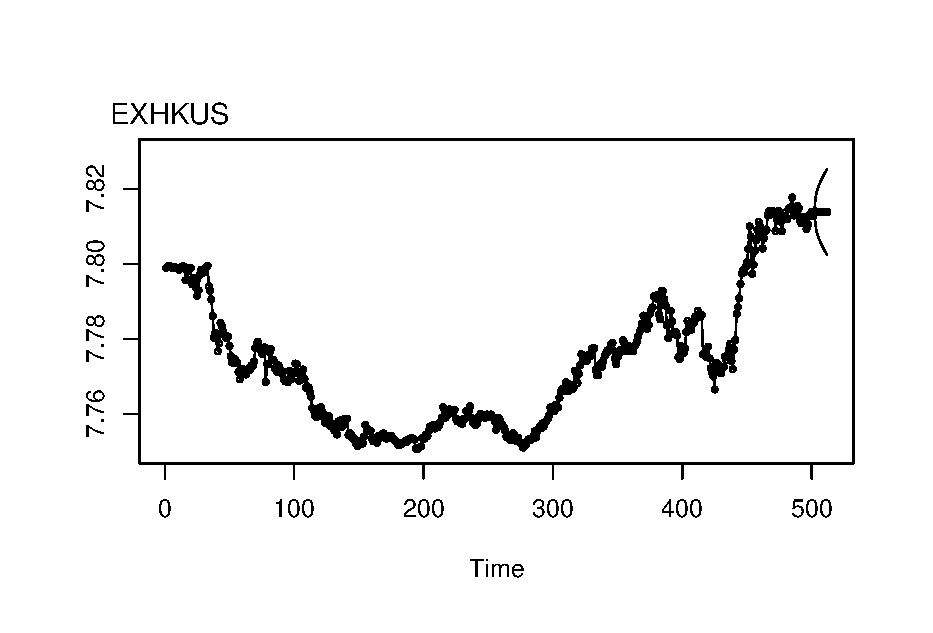
\includegraphics[width=.8\textwidth]{Chapter8AutoReg/F88ARI21Fore.eps}
    \caption{\label{F8:HKForecast} \small Ten Day Forecasts and Forecast Intervals of the Hong Kong Exchange Rates.
    Forecasts are based on the ARIMA(2,1,0) model.}
  \end{center}
\end{figure}

\linejed
\bigskip



\section{Further Reading and References}

The classic book-long introduction to Box-Jenkins time series is
Box, Jenkins and Reinsel (1994).

\bigskip


\textbf{Chapter References}

\begin{multicols}{2}

\scalefont{0.9}

Abraham, Bovas and  Johannes Ledolter (1983). \textit{Statistical
Methods for Forecasting}. John Wiley \& Sons, New York.

Box, George E. P., Gwilym M. Jenkins and Gregory C. Reinsel (1994).
\textit{Time Series Analysis: Forecasting and Control}, Third
Edition, Prentice-Hall, Englewood Cliffs, New Jersey.

Box, George E. P., and D. A. Pierce (1970). Distribution of residual
autocorrelations in autoregressive moving average time series
models. \textit{Journal of the American Statistical Association} 65,
1509-1526.

Chan, Wai-Sum and Siu-Hang Li (2007). The Lee-Carter model for
forecasting mortality, revisited. \textit{North American Actuarial
Journal} 11(1), 68-89.

Lee, Ronald D. and Lawrence R. Carter (1992). Modelling and
forecasting U.S. mortality. \textit{Journal of the American
Statistical Association} 87, 659-671.

Ljung, G. M. and George E. P. Box (1978). On a measure of lack of
fit in time series models. \textit{Biometrika} 65, 297-303.

MacLeod, A. I. (1977). Improved Box-Jenkins estimators.
\textit{Biometrika} 64, 531-534.

MacLeod, A. I. (1978). On the distribution of residual
autocorrelations in Box-Jenkins models. \textit{Journal of the Royal
Statistical Society B} 40, 296-302.

Miller, Robert B. and Dean W. Wichern (1977). \emph{Intermediate
Business Statistics: Analysis of Variance, Regression and Time
Series}. Holt, Rinehart and Winston, New York.

Roberts, Harry V. (1991). \emph{Data Analysis for Managers with
MINITAB}. Scientific Press, South San Francisco, CA.

\scalefont{1.1111}

\end{multicols}

\section{Exercises}

\scalefont{0.90}
\begin{exercises}

\item A mutual fund has provided investment yield rates for five consecutive years as follows:
\begin{center}
\begin{tabular}{lccccc}
  \hline
 Year & 1 & 2 & 3 & 4 & 5 \\
Yield & 0.09 & 0.08 & 0.09 & 0.12 & -0.03 \\
  \hline
\end{tabular}\end{center}

Determine $r_1$ and $r_2$, the lag 1 and lag 2 autocorrelation
coefficients.

\item The \textit{Durbin-Watson} statistic is designed to detect autocorrelation and is defined by:
\begin{equation*}
DW = \frac {\sum_{t=2}^T (y_t - y_{t-1})^2} {\sum_{t=1}^T (y_t -
\bar{y})^2}.
\end{equation*}\index{time series
statistics!Durbin-Watson}


a. Derive the approximate relationship between $DW$ and the lag 1
autocorrelation coefficient $r_1$.

b. Suppose that $r_1 = 0.4$. What is the approximate value of $DW$?



\item Consider the Chapter 2 linear regression model formulas with
$y_{t-1}$ in place of $x_t$, for $t=2, \ldots, T$.

a. Provide an exact expression for $b_1$.

b. Provide an exact expression for $b_0$.

c. Show that $b_0 \approx \bar{y} (1-r_1) $.

\item Begin with the $AR$(1) model as in equation (\ref{E8:AR1}).

a. Take variances of each side of equation (\ref{E8:AR1}) to show
that $\sigma_y^2(1-\beta_1^2) = \sigma^2,$ where $\sigma_y^2 =
\mathrm{Var}~y_t$ and $\sigma^2 = \mathrm{Var}~\varepsilon_t$.

b. Show that $\mathrm{Cov}(y_t,y_{t-1}) = \beta_1 \sigma_y^2.$

c. Show that $\mathrm{Cov}(y_t,y_{t-k}) = \beta_1^k \sigma_y^2.$

d. Use part (c) to establish equation
(\ref{E8:AR1Autocorrelations}).

\item Consider forecasting with the $AR$(1) model.

a. Use the forecasting chain rule in equation (\ref{E8:ChainRule})
to show
\begin{equation*}
y_{T+k}-\widehat{y}_{T+k} \approx \varepsilon_{T+k} + \beta_1
\varepsilon_{T+k-1} + \cdots + \beta_1^{k-1} \varepsilon_{T+1}.
\end{equation*}

b. From part (a), show that the approximate variance of the forecast
error is $\sigma^2 \sum_{l=0}^{k-1} \beta_1^{2l}.$


\index{datasets!Standard and Poor's daily
returns}\empexjed{SP500Daily}
\item These data consist of the 503 daily returns for the calendar
years 2005 and 2006 of the Standard and Poor's (S\&P) value weighted
index. (The data file contains additional years - this exercise uses
only 2005 and 2006 data.) Each year, there are about 250 days on
which the exchange is open and stocks were traded - on weekends and
holidays it is closed. There are several indices to measure the
market's overall performance. The \textit{value weighted index} is
created by assuming that the amount invested in each stock is
proportional to its market capitalization. Here, the market
capitalization is simply the beginning price per share times the
number of outstanding shares. An alternative is the \textit{equally
weighted index}, created by taking a simple average of the closing,
or last, price of stocks that form the S\&P on that trading day.

Financial economic theory states that if the market were predictable, many
investors would attempt to take advantage of these predictions, thus forcing
unpredictability. For example, suppose a statistical model reliably
predicted mutual fund A to increase two-fold over the next 18 months. Then,
the no arbitrage principle in financial economics states that several alert
investors, armed with information from the statistical model, would bid to
buy mutual fund A, thus causing the price to increase because demand is
increasing. These alert investors would continue to purchase until the price
of mutual fund A rose to the point where the return was equivalent to other
investment opportunities in the same risk class. Thus, any advantages
produced by the statistical model would disappear rapidly, thus eliminating
this advantage.

Thus, financial economic theory states that for liquid markets such
as stocks represented through the S\&P index there should be no
detectable patterns, resulting in a white noise process. In
practice, it has been found that cost of buying and selling equities
(called transactions costs) are large enough so as to prevent us
from taking advantage of these slight tendencies in the swings of
the market. This illustrates a point known as \emph{statistically
significant but not practically important}. This is not to suggest
that statistics is not practical (heavens forbid!). Instead,
statistics in and of itself does not explicitly recognize factors,
such as economic, psychological and so on, that may be extremely
important in any given situation. It is up to the analyst to
interpret the statistical analysis in light of these
factors.\bigskip


\begin{figure}[htp]
  \begin{center}
   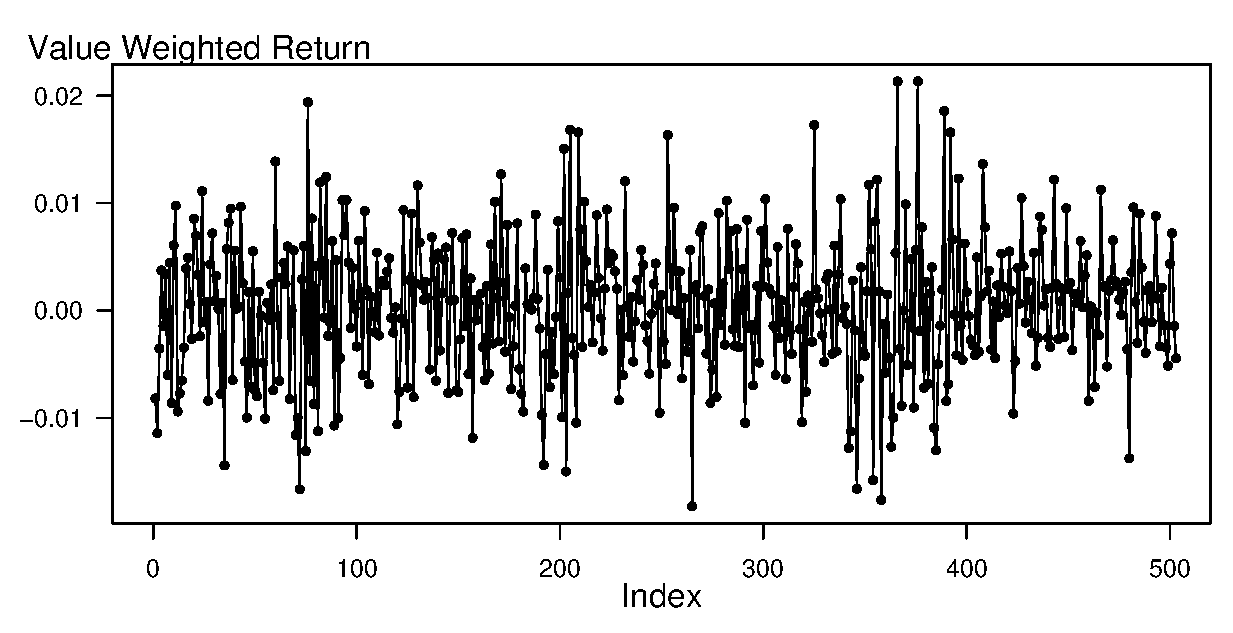
\includegraphics[width=.8\textwidth]{Chapter8AutoReg/ValueWgtReturn.eps}
      \caption{\label{F8:SPValue} \small Time Series Plot of the S \& P Daily Market Return, 2005-2006.}
      \end{center}
\end{figure}


a. The time series plot in Figure \ref{F8:SPValue} gives a
preliminary idea of the characteristics of the sequence. Comment on
the stationarity of the sequence.

b. Calculate summary statistics of the sequence. Suppose that you assume a
white noise model for the the sequence. Compute 1, 2 and 3 step ahead
forecasts for the daily returns for the first three trading days of 2007.

c. Calculate the autocorrelations for the lags 1 through 10. Do you detect
any autocorrelations that are statistically significantly different from
zero?


\end{exercises}
\scalefont{1.1111}
